\section{Signal Intepretations}
The signal hypotheses targetted in this search are provided under a set of simplified mediator models. These models assume an additional particle, 
a fermionic dark matter candidate, and an additional interaction that forces the production of a dark matter. 
For generality, it is assumed that this additional interaction is mediated by a generic spin-0 or spin-1 particle. 
The interactions are characterised by four distinct Lagrangians, written for a Dirac-fermion dark matter particle $\chi$ as, 

\begin{align}
\label{eq:LS} 
\mathcal{L}_{\mathrm{scalar}}&\supset\, -\,\frac{1}{2}m_{\rm MED}^2 S^2 - g_{\rm DM}  S \, \bar{\chi}\chi
 - \sum_{q=b,t} g_{SM}^q S \, \bar{q}q  - m_{\rm DM} \bar{\chi}\chi \,,
 \\
 \label{eq:LP} 
\mathcal{L}_{\rm{pseudo-scalar}}&\supset\, -\,\frac{1}{2}m_{\rm MED}^2 P^2 - i g_{\rm DM}  P \, \bar{\chi} \gamma^5\chi
 -\sum_{q=b,t}  i g_{SM}^q  P \, \bar{q}  \gamma^5q  - m_{\rm DM} \bar{\chi}\chi\,,
 \\
 \label{eq:LV} 
\mathcal{L}_{\mathrm{vector}}&\supset \, \frac{1}{2}m_{\rm MED}^2 Z'_{\mu} Z'^{\mu} - g_{\rm DM}Z'_{\mu} \bar{\chi}\gamma^{\mu}\chi -\sum_q g_{SM}^q Z'_{\mu} \bar{q}\gamma^{\mu}q - m_{\rm DM} \bar{\chi}\chi\,,
 \\
 \label{eq:LA} 
\mathcal{L}_{\rm{axial}}&\supset\,  \frac{1}{2}m_{\rm MED}^2 Z''_{\mu} Z''^{\mu} - g_{\rm DM} Z''_{\mu} \bar{\chi}\gamma^{\mu}\gamma^5\chi -\sum_q g_{SM}^q Z''_{\mu} \bar{q}\gamma^{\mu}\gamma^5q - m_{\rm DM} \bar{\chi}\chi\,
\end{align}

assuming pure scalar, psuedoscalar, axial-vector and vector mediated interactions denoted by $S,~P,~Z'$ and $Z''$ mediators respectively. 
The couplings $g_{DM}$ and $g_{SM}$ denotes the coupling of the mediator to the dark matter particle and to standard model particles respectively. 
The choice of this split in the Lagrangian is to parallel the existing separation with direct detection, into spin-dependent and spin-independent interactions. 
Here, spin-independent can refer to either vector or scalar mediated interactions, between which direct detection makes no distinction, while 
spin-dependent interactions refer to axial-vector mediated processes. 
Pseudoscalar interactions are velocity suppressed in DM-nucleon interactions and thus limited sensitivity from the direct detection experiments is expected~\cite{Haisch:2012kf}. 
An extension to the scalar and pseudo-scalar can be performed by allowing the (pseudo-)scalar interactions to undergo electroweak symmetry breaking (EWSB) in an analogous way to 
the Higgs mechanism~\cite{Khoze:2015sra,Hambye:2013sna,Khoze:2014xha,Khoze:2014woa,Altmannshofer:2014vra,Carone:2013wla,Heikinheimo:2013fta}. Scalar and pseudoscalar models 
where EWSB is not present are denoted herein as \emph{fermionic} dark matter production.

In collider experiments, the production of dark matter in spin-0 mediated interactions is predominantly through gluon-fusion via a top-quark loop. 
When EWSB is present in the model, mono-V signatures are produced through the well known higgs-strahlung 
process(figure~\ref{fig:monoXfeyn}). For the spin-1 signatures, dark matter is produced in an analogous way to Z boson production through quark initiated processes. The mono-V or monojet signatures follow 
from the presence of a radiated V-boson or jet in the initial state. In all models, the coupling of the mediator to standard model coupling is taken as unity 
($g_{SM}=1$) along with 
the dark matter coupling ($g_{DM}=1$). For the (pseudo-)scalar models, this denotes a Yukawa coupling to standard model particles. For all models considered, 
the width is fixed under the minimum width constraint~\cite{Harris:2014hga}.

In order to model the expected contribution from these signals, Monte Carlo (MC) events are generated using MCFM~\cite{mcfm}
for the monojet final state, and JHUGen~\cite{Anderson:2013afp} 
for the vector boson final state. All signal models are 
generated at leading order, showered with Pythia6 and passed through a 
simulation of the CMS detector using Geant4~\cite{geant4}. 
For scalar and pseudoscalar mediated DM production, the finite top mass is 
taken into account. 

\begin{figure}[htbp]
  \centering
  \subfloat[][]{
        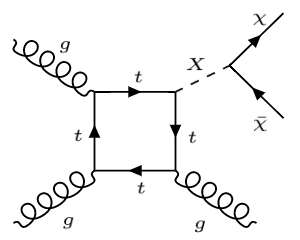
\includegraphics[angle=0,width=0.36\textwidth]{figures/scalarbox.png}
        \label{fig:monojet0}
  }
  \subfloat[][]{
        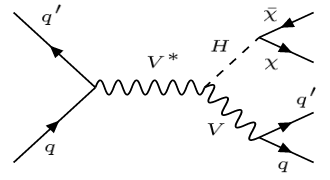
\includegraphics[angle=0,width=0.36\textwidth]{figures/scalarV.png}
        \label{fig:monoV0}
  }
  \caption{Diagrams for production of the monojet (a) and mono-V signature through Higgs-strahlung (b), through a scalar mediator.\label{fig:monoXfeyn}}
\end{figure}



